\chapter{Results}
\label{chp5:results} 
In this chapter we present our results we have gained from our empirical research. 
We first present our result from the Knowles microphone.

After the Knowles results, we list the results that are produced in accordance with the experimental plan in~\autoref{apx:experiment_plan}. 
These results are from the anechoic chamber and the associated results from an office environment.  
We will first present the results gained from the microinstructions, followed by the results from CPU load and decryption. 

%===================================================================================================================
%                                               Knowles microphone
%===================================================================================================================
\section{Results from Knowles}\label{chp5:sec:knowles_results}
The results from the Knowles microphone are gained when experimenting with different types of setups.
The recordings are done in a try and fail approach rather than according to an experimental plan.

\subsection{Results from Lenovo T60p - decryption}\label{chp5:subsec:t60p_knowles_results_decryption}
In~\autoref{fig:T60p-knowles-decrypt-ips} we ran the decryption specified in~\autoref{chp4:sec:decryption}. 
In~\autoref{fig:T60p-knowles-decrypt-ips-2} we ran a different decryption setup, described in~\autoref{lst:decryption_loop}.

\begin{lstlisting}[
language=BASH, 
caption={Decryption of an image file.}, 
label={lst:decryption_loop}]
sleep 1             
gpg --output tmp/image_de.png --decrypt img.gpg
sleep 1
gpg --output tmp/image_de2.png --decrypt img.gpg
sleep 1
gpg --output tmp/image_de3.png --decrypt img.gpg
gpg --output tmp/image_de4.png --decrypt img.gpg    
gpg --output tmp/image_de5.png --decrypt img.gpg
gpg --output tmp/image_de6.png --decrypt img.gpg
\end{lstlisting}

%================
% T60p deryption
%================
\begin{figure}[ht]
    \begin{subfigure}{0.5\textwidth}
        \centering
        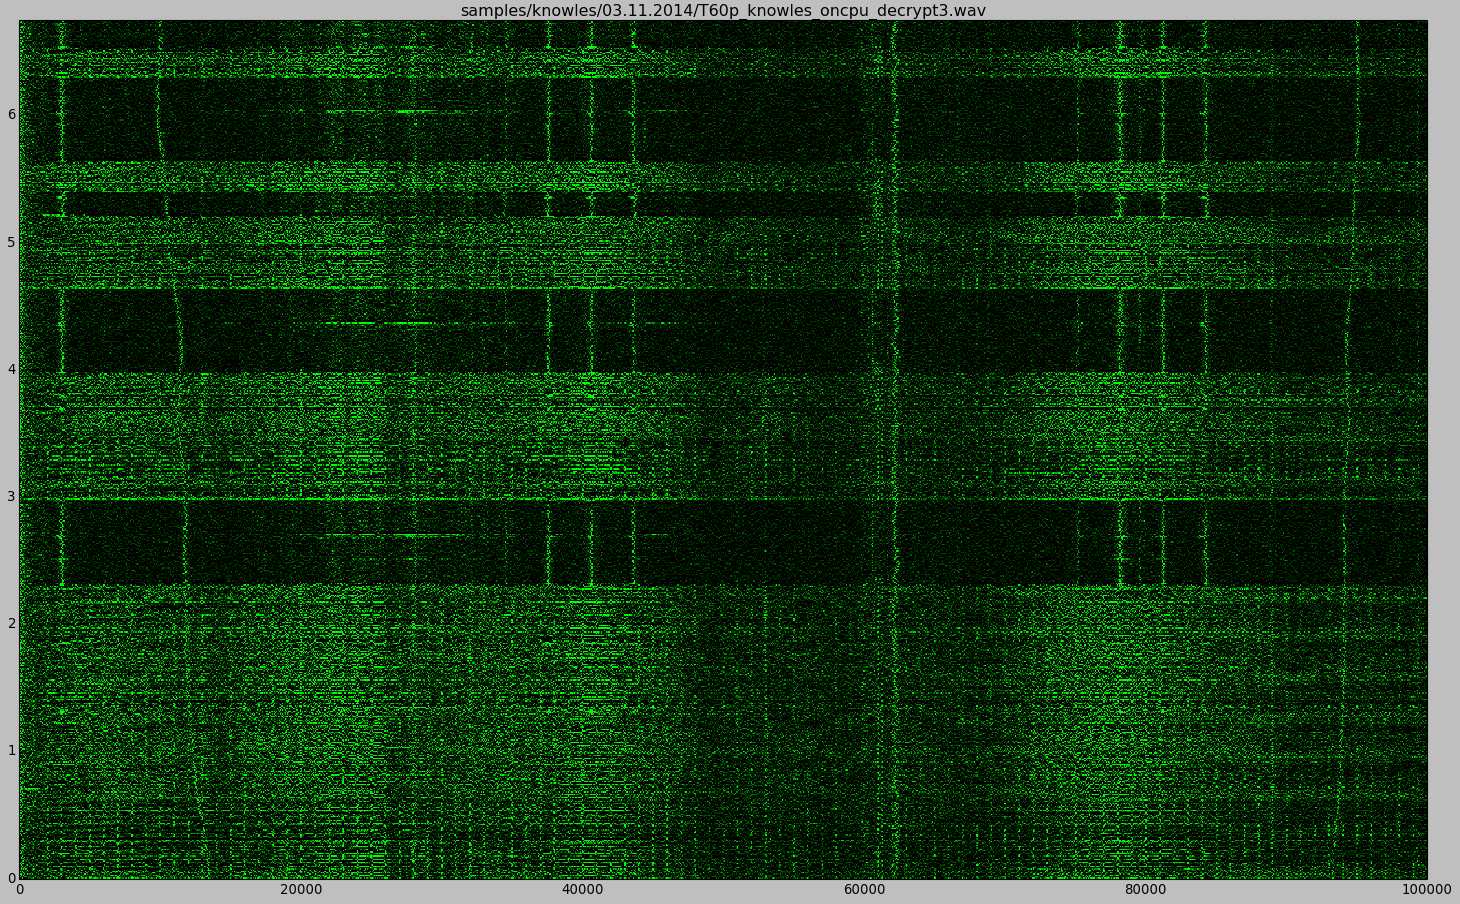
\includegraphics[width=1\linewidth]{T60p-knowles-decrypt-ips.png}
        \caption{}
        \label{fig:T60p-knowles-decrypt-ips}
    \end{subfigure}
    \begin{subfigure}{0.5\textwidth}
        \centering
        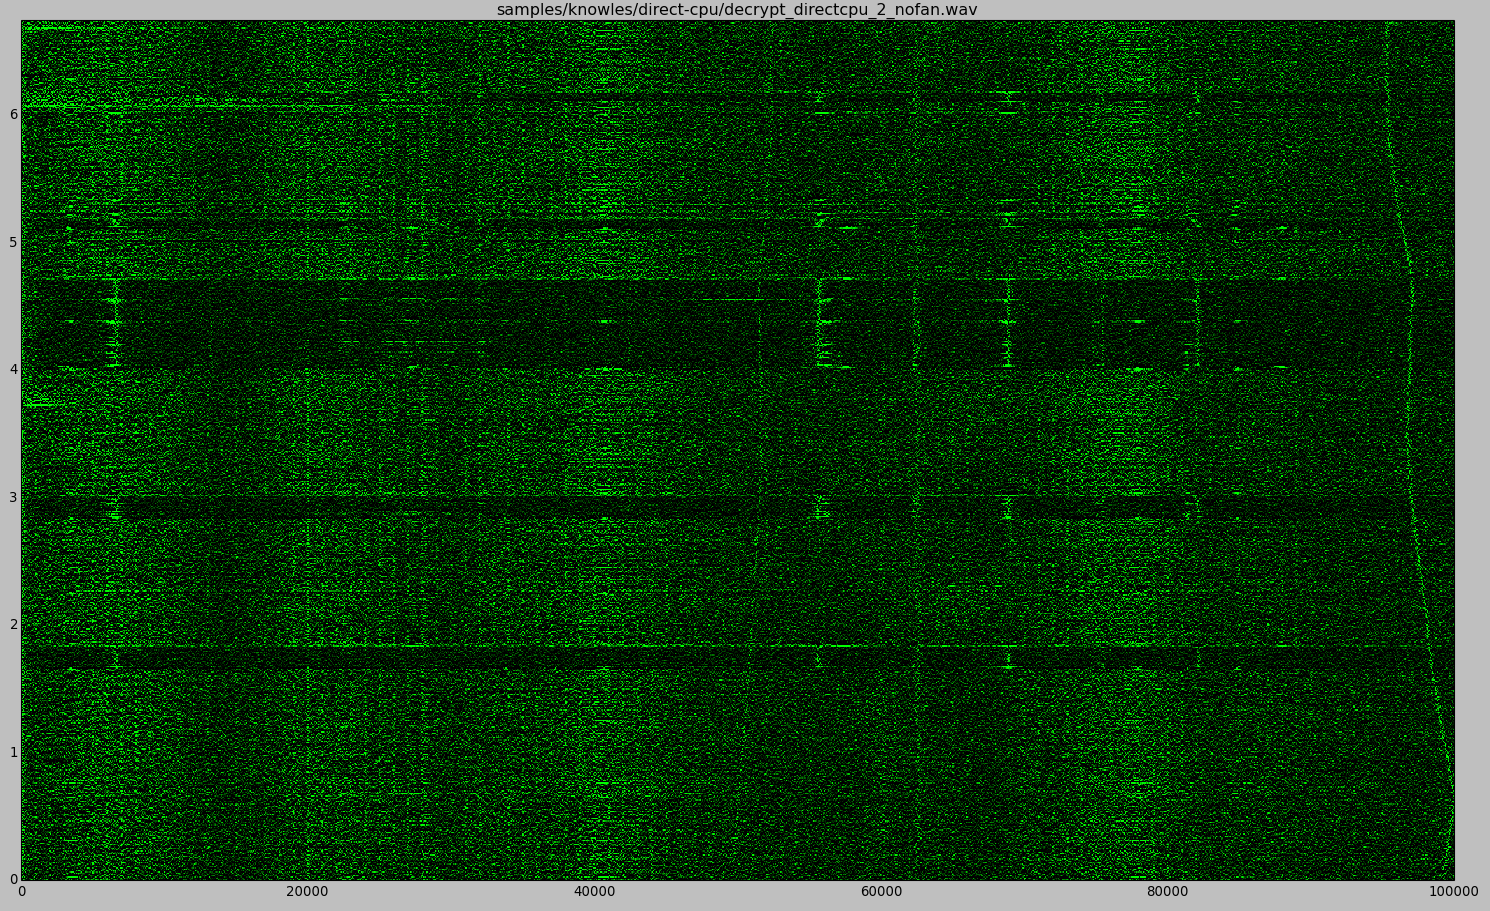
\includegraphics[width=1\linewidth]{T60p-knowles-decrypt-ips-2.png}
        \caption{}
        \label{fig:T60p-knowles-decrypt-ips-2}
    \end{subfigure}
    \caption{Acoustic recording (Vertical axis: 7 sec. Horizontal axis: 0-100kHz) of the Lenovo T60p when running decryption.
    Both recordings was made in an office environment using the Knowles configuration specified in~\autoref{ch3:sec:knowles_configuration} and running on battery power. }
    \label{fig:T60p-knowles-decrypt-ips}
\end{figure}

%================
% T60p micro
%================
\subsection{Results from Lenovo T60p - microinstructions}\label{chp5:subsec:t60p_knowles_results_micro}
The plot in~\autoref{fig:T60p-knowles-micro-ips-0} and has been produced using a different approach with regard to the signal processing. 
Since we are not required to transform the sound file back to the time domain, we are able to sample overlapping windows.
In the case of this plot, we are taking the fourier transform of windows of size 2048 samples, but only moving the sliding window \({W/2}\) samples.
Additionally, the plot shows the 10th logarithm of the frequency responses, and only values between the median value (min) and 0 (max) are indicated with the colors (in a linear scale, as in the other plots). 
\begin{figure}[ht]
    \centering
    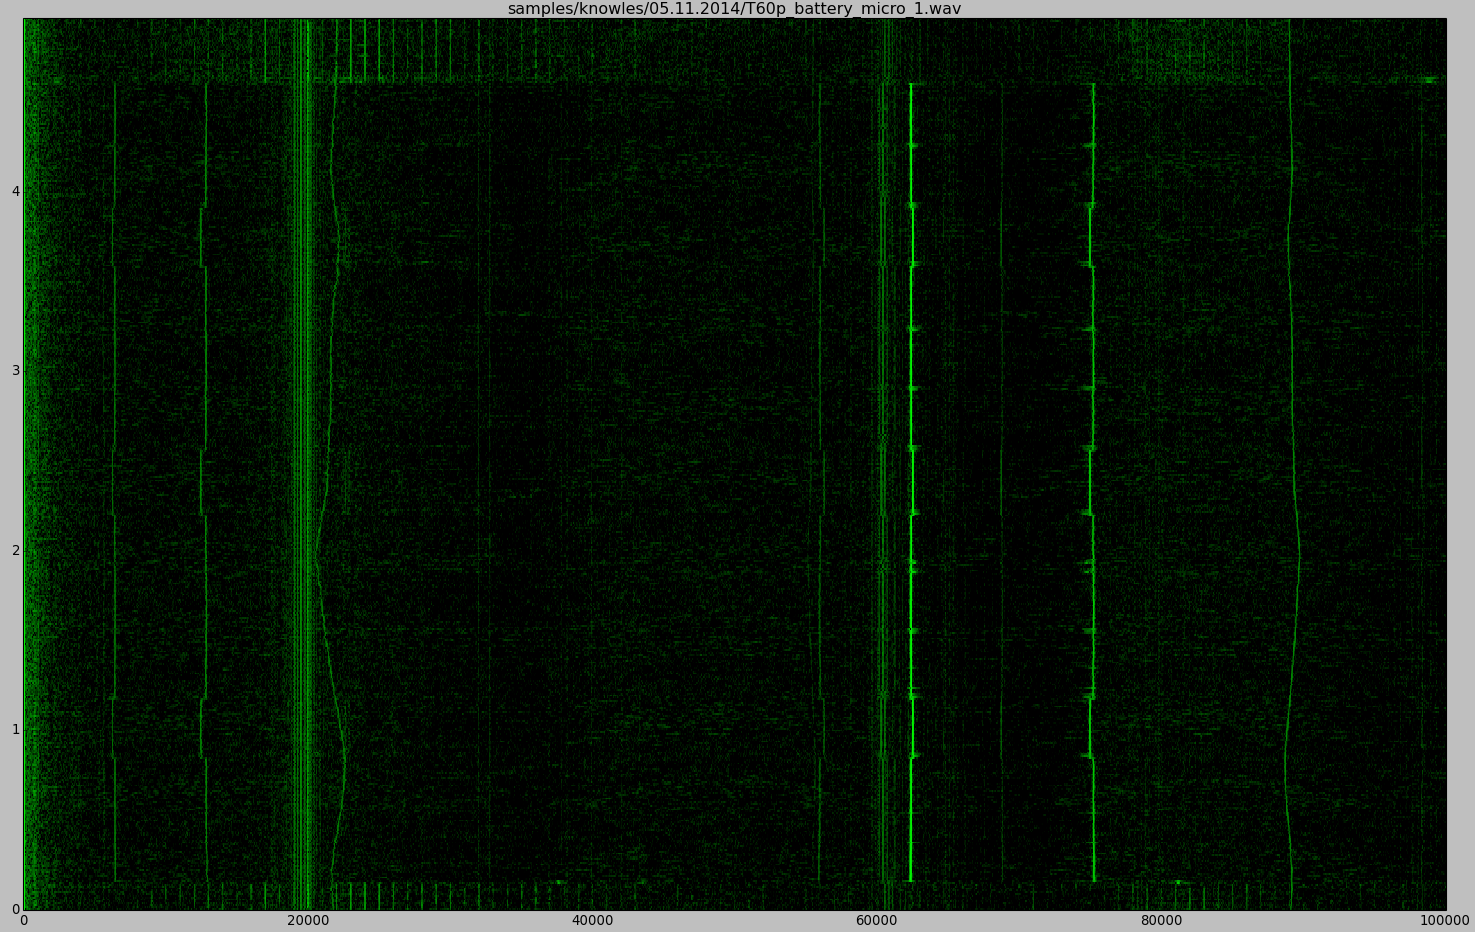
\includegraphics[width=0.6\linewidth]{T60p-knowles-micro-ips-0.png}
    \caption{Acoustic recording (Vertical axis: 5 sec. Horizontal axis: 0-100kHz) of the Lenovo T60p when running microinstructions described in~\autoref{chp4:sec:microinstructions}. The recording was made in an office environment using the Knowles configuration specified in~\autoref{ch3:sec:knowles_configuration} and running on battery power. }
    \label{fig:T60p-knowles-micro-ips-0}
\end{figure}
%================
% T60p CPU load
%================
\subsection{Results from Lenovo T60p - CPU load}\label{chp5:subsec:t60p_knowles_results_cpuload}
The plot in~\autoref{fig:T60p-knowles-cpuload-ips-0} has been produced running full CPU load.
In~\autoref{fig:T60p-knowles-cpuload-ips-0} is the result gained from running a full CPU load in the Lenovo T60p computer. 
\begin{figure}[ht]
    \centering
    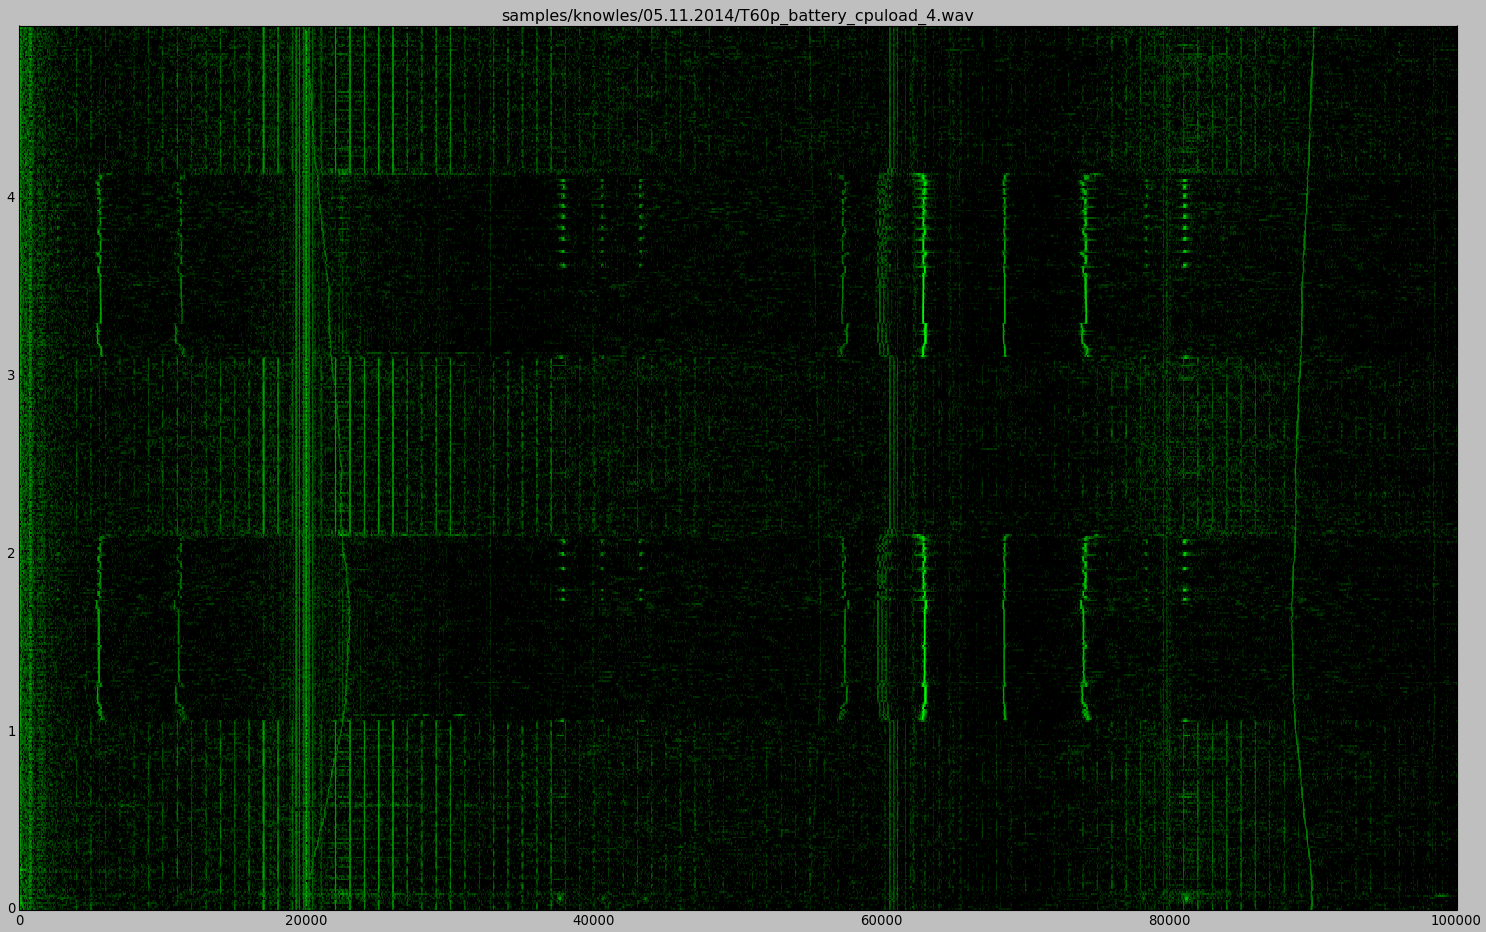
\includegraphics[width=0.6\linewidth]{T60p-knowles-cpuload-ips-0.png}
    \caption{Acoustic recording (Vertical axis: 5 sec. Horizontal axis: 0-100kHz) of the Lenovo T60p when running a full CPU load described in~\autoref{chp4:sec:cpu_load}. The recording was made in an office environment using the Knowles configuration specified in~\autoref{ch3:sec:knowles_configuration} and running on battery power. }
    \label{fig:T60p-knowles-cpuload-ips-0}
\end{figure}

%===================================================================================================================
%                                               Brüel&Kjær microphone
%===================================================================================================================
%=============
% T60p MICRO
%=============
\section{Results from Brüel\&Kjær}\label{chp5:sec:bk_results}
In this section we present the results gained from the Brüel\&Kjær configuration specified in~\autoref{ch3:sec:bruel_kjaer_configuration}. 
In contrast to the results presented in~\autoref{chp5:sec:knowles_results}, these experiments are carefully done according to the experimental plan described in in~\autoref{apx:experiment_plan}. 

\subsection{Results from Lenovo T60p - microinstructions}\label{chp5:subsec:t60p_bk_results_micro}
The~\autoref{fig:T60p-ekkofritt-bk-micro-eps-1} and the~\autoref{fig:T60p-ekkofritt-bk-micro-ips-3} is the result from doing the microinstructions described in~\autoref{chp4:sec:microinstructions} in the anechoic chamber on the Lenovo T60p computer.
%=============================
% T60p Anechoic chamber MICRO
%=============================
\begin{figure}[ht]
	\begin{subfigure}{0.5\textwidth}
	    \centering
	    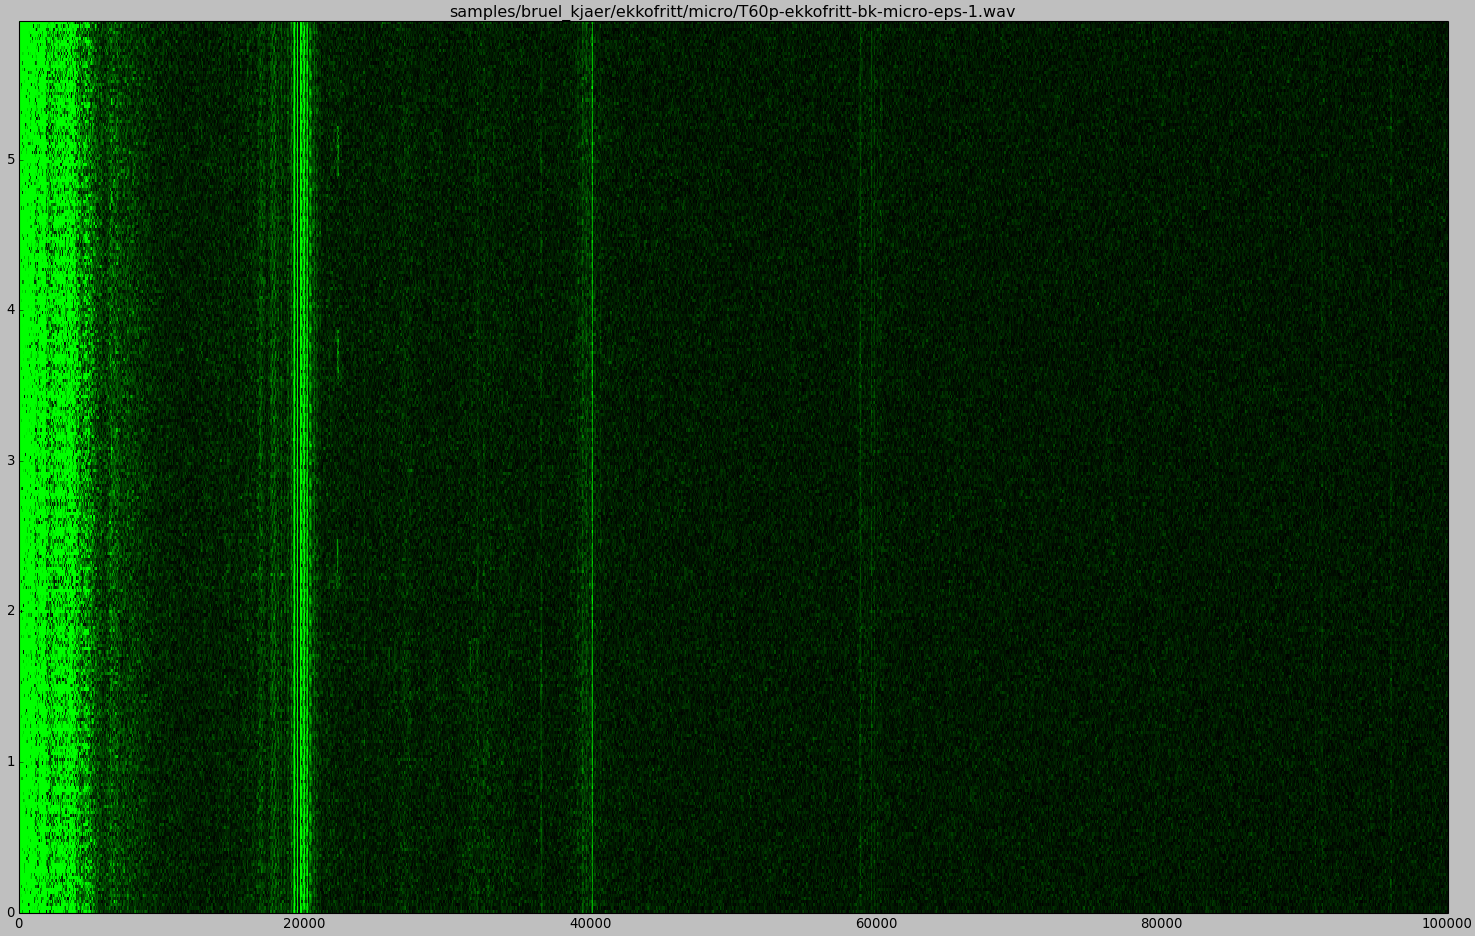
\includegraphics[width=1\linewidth]{T60p-ekkofritt-bk-micro-eps-1.png}
	    \caption{With power adopter}
	    \label{fig:T60p-ekkofritt-bk-micro-eps-1}
    \end{subfigure}
    \begin{subfigure}{0.5\textwidth}
	    \centering
    	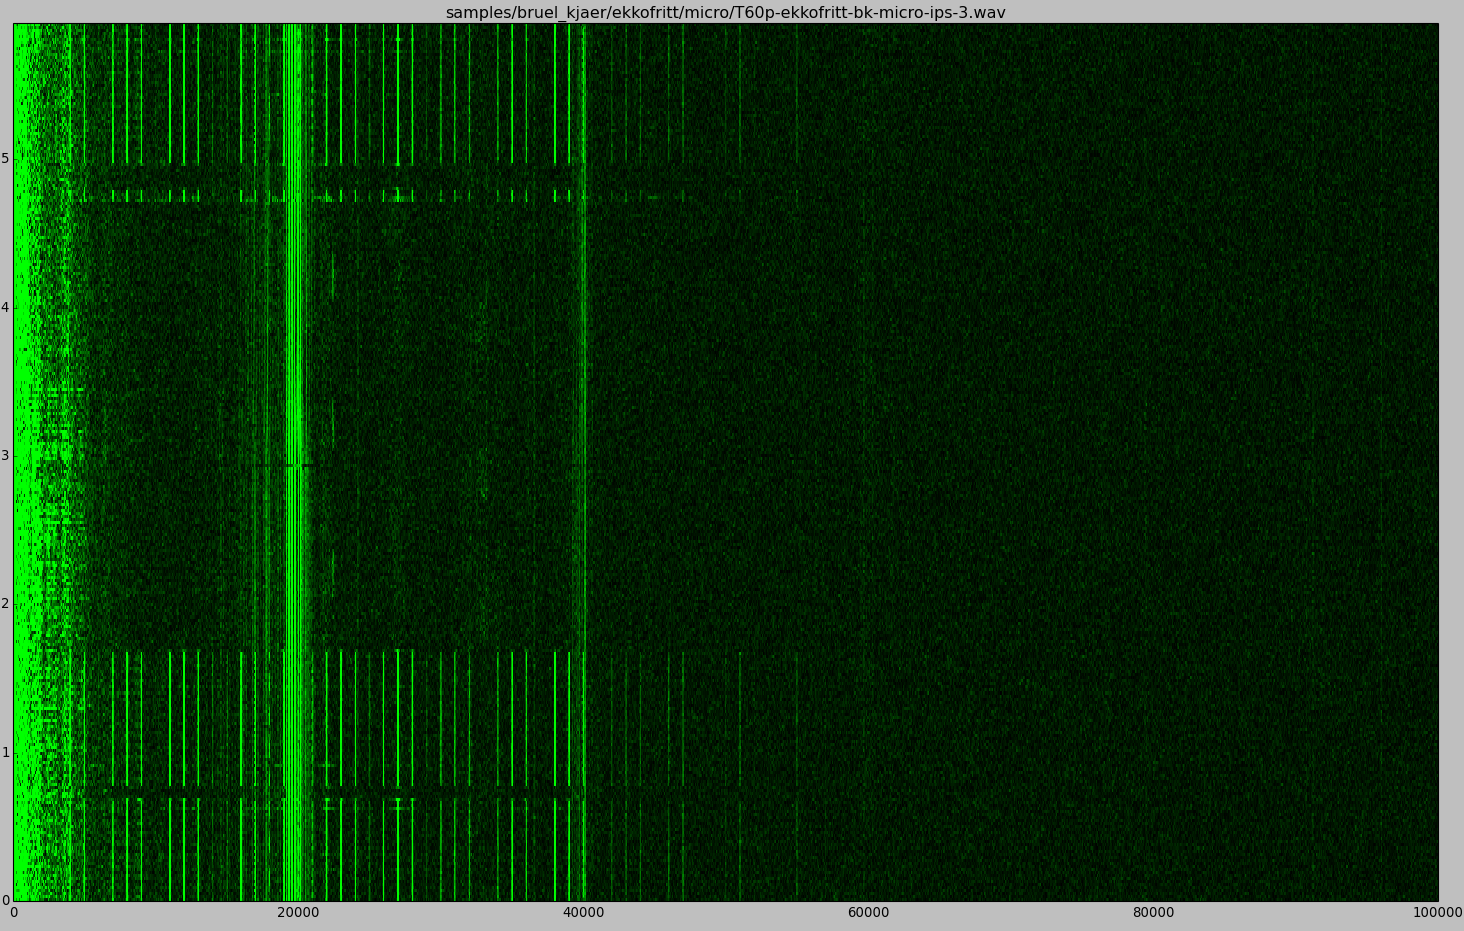
\includegraphics[width=1\linewidth]{T60p-ekkofritt-bk-micro-ips-3.png}
    	\caption{Running on battery power}
    	\label{fig:T60p-ekkofritt-bk-micro-ips-3}
    \end{subfigure}
    \caption{Acoustic recording (Vertical axis: 6 sec. Horizontal axis: 0-100kHz) of the Lenovo T60p when running microinstructions described in~\autoref{chp4:sec:microinstructions}. Both recordings was made in an anechoic chamber using the Brüel\&Kjær 4939 configuration specified in~\autoref{ch3:sec:bruel_kjaer_configuration}. }
	\label{fig:T60p-ekkofritt-bk-micro}
\end{figure}
%==========================
% T60p Normal room MICRO
%==========================
The~\autoref{fig:T60p-bk-micro-ips-0} is the same recordings as in~\autoref{fig:T60p-ekkofritt-bk-micro}, but in an office environment.
\begin{figure}[ht]
    \centering
    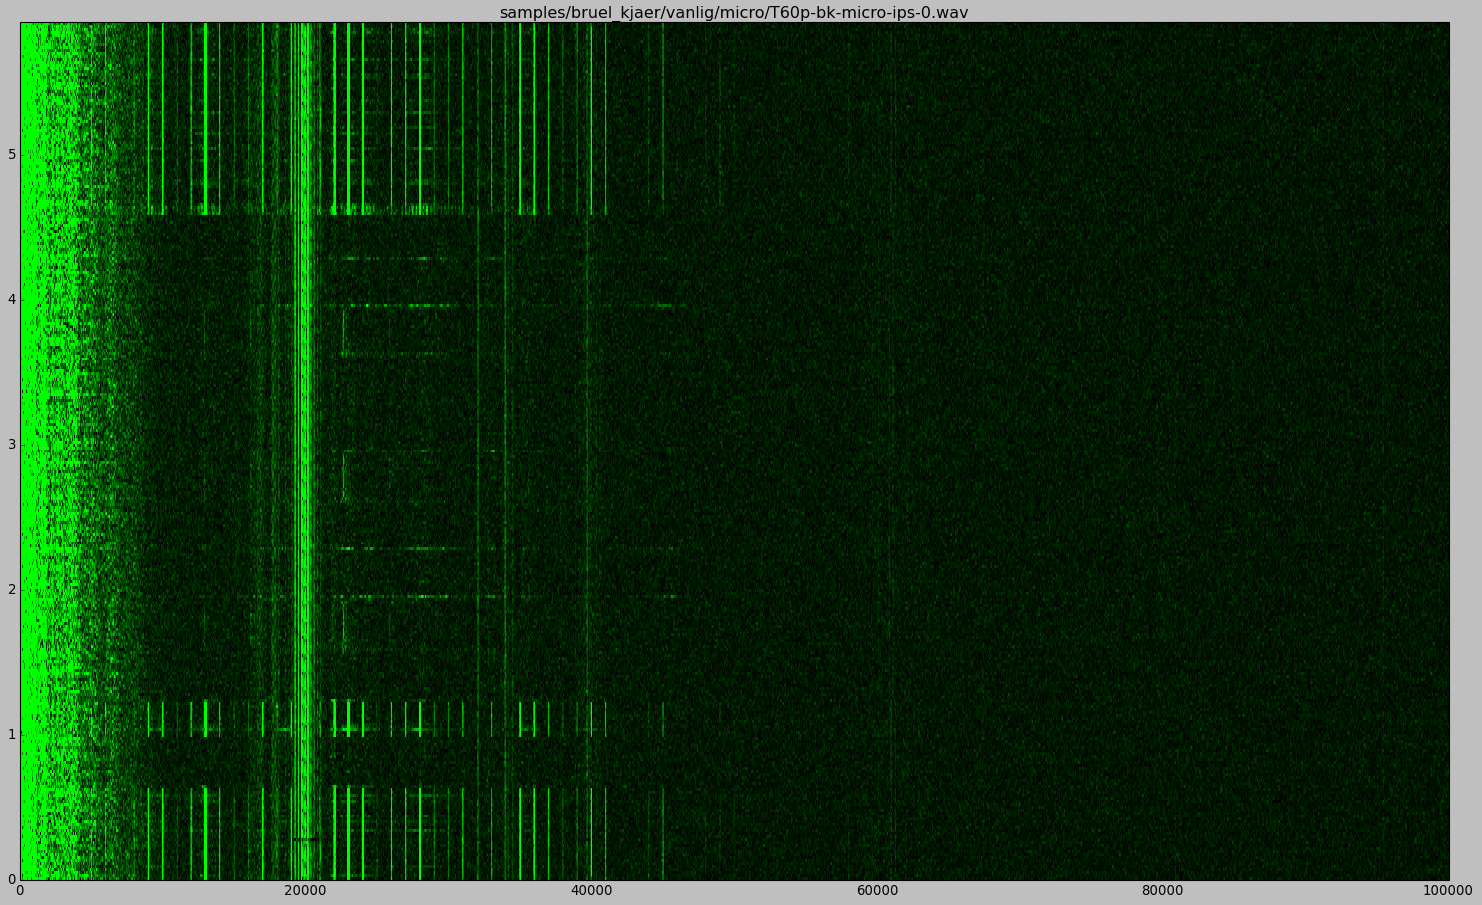
\includegraphics[width=0.7\linewidth]{T60p-bk-micro-ips-0.png}
    \caption{Acoustic recording (Vertical axis: 6 sec. Horizontal axis: 0-100kHz) of the Lenovo T60p when running microinstructions described in~\autoref{chp4:sec:microinstructions}. The recording was made using the Brüel\&Kjær 4939 configuration specified in~\autoref{ch3:sec:bruel_kjaer_configuration}. }
    \label{fig:T60p-bk-micro-ips-0}
\end{figure}

%==============
% T60p CPULOAD
%==============
\subsection{Results from Lenovo T60p - CPU load}\label{chp5:subsec:t60p_bk_results_cpuload}
The~\autoref{fig:T60p-ekkofritt-bk-cpuload-eps-4} and the~\autoref{fig:T60p-ekkofritt-bk-cpuload-ips-0} is the results from the running CPU load on the Lenovo T60p in the anechoic chamber. 
%===============================
% T60p Anechoic chamber CPULOAD
%===============================

\begin{figure}[ht]
	\begin{subfigure}{0.5\textwidth}
	    \centering
	    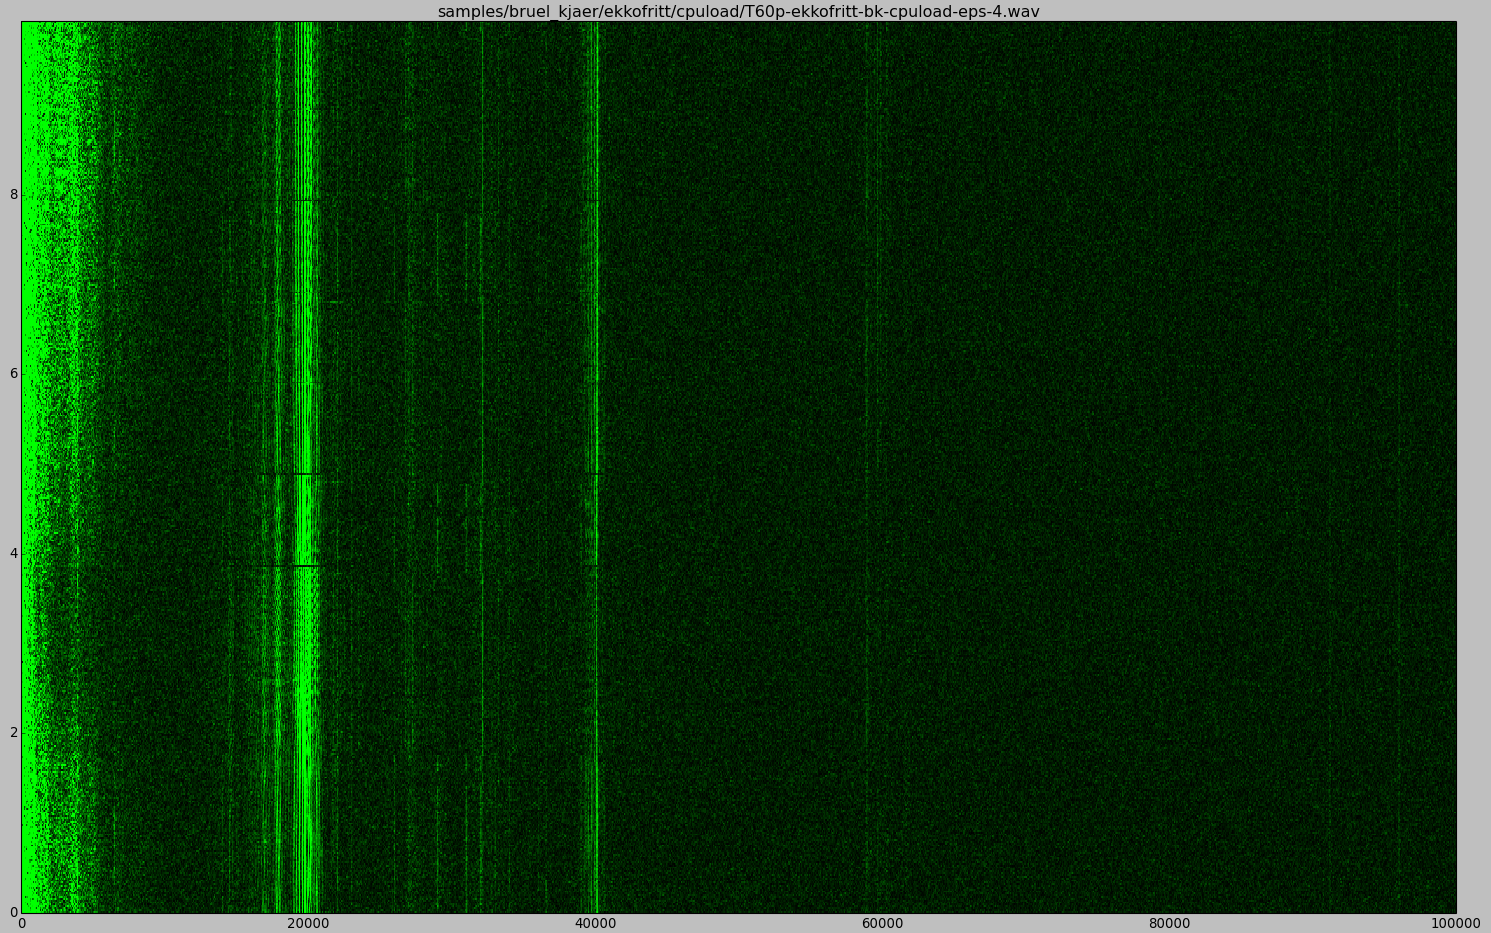
\includegraphics[width=1\linewidth]{T60p-ekkofritt-bk-cpuload-eps-4.png}
	    \caption{With power adopter}
	    \label{fig:T60p-ekkofritt-bk-cpuload-eps-4}
    \end{subfigure}
    \begin{subfigure}{0.5\textwidth}
	    \centering
	    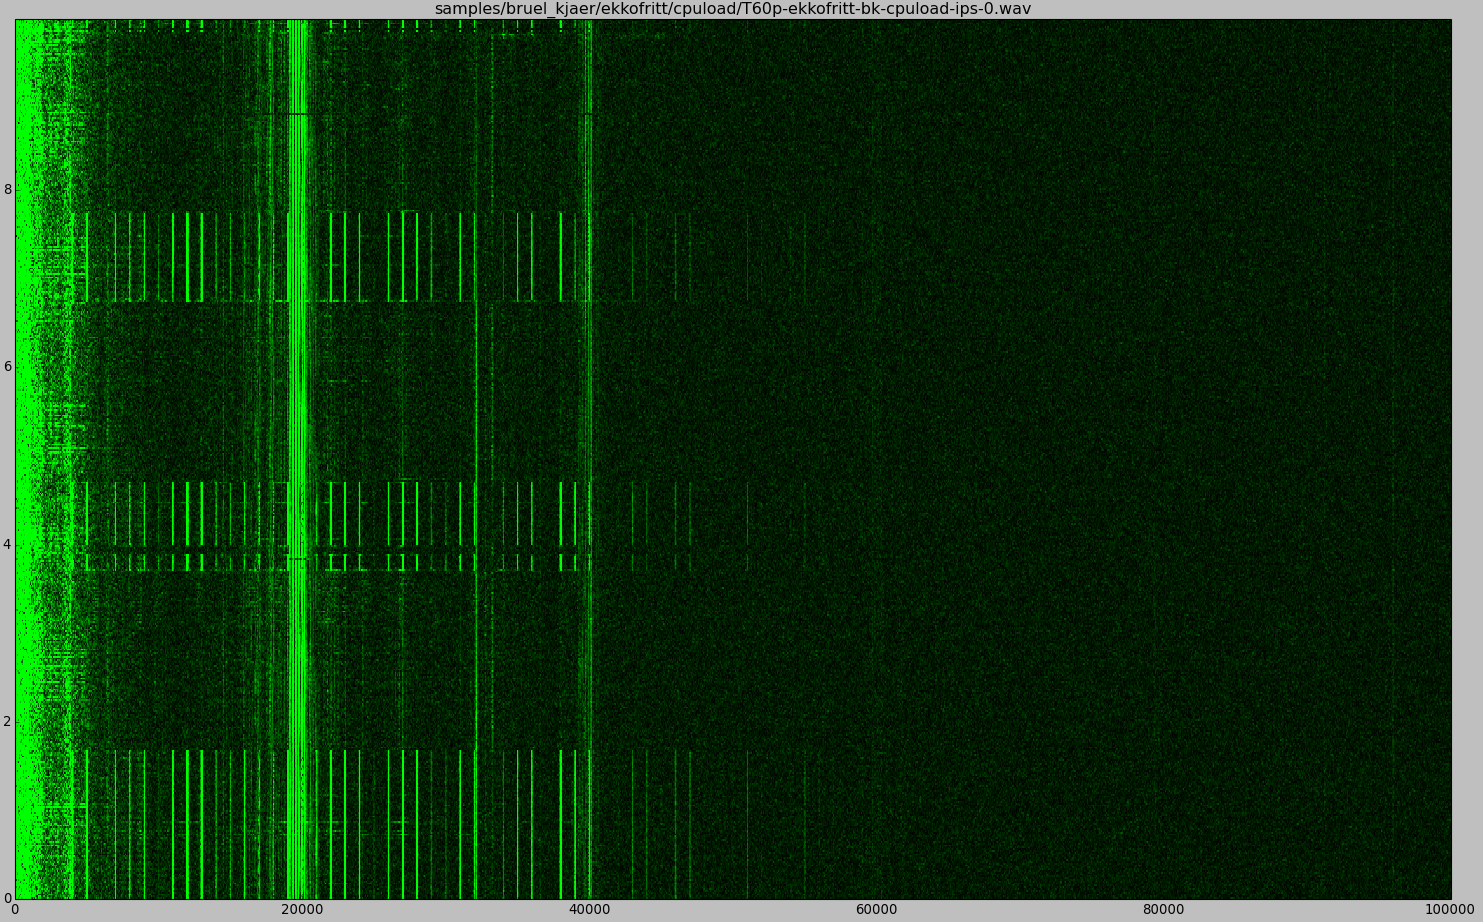
\includegraphics[width=1\linewidth]{T60p-ekkofritt-bk-cpuload-ips-0.png}
	    \caption{Running on battery power}
	    \label{fig:T60p-ekkofritt-bk-cpuload-ips-0}
    \end{subfigure}
    \caption{Acoustic recording (Vertical axis: 10 sec. Horizontal axis: 0-100kHz) of the Lenovo T60p when running a full CPU load described in~\autoref{chp4:sec:cpu_load}. The recording was made in an anechoic chamber using the Brüel\&Kjær 4939 configuration specified in~\autoref{ch3:sec:bruel_kjaer_configuration}.}
	\label{fig:T60p-ekkofritt-bk-cpuload}
\end{figure}
%==========================
% T60p Normal room CPULOAD
%==========================
The~\autoref{fig:T60p-bk-cpuload-eps-1-1a} and the~\autoref{fig:T60p-bk-cpuload-ips-0-1b} is the results from the running CPU load, described in~\autoref{chp4:sec:cpu_load}, on the Lenovo T60p in an office environment. 
\begin{figure}[ht]
	\begin{subfigure}{0.5\textwidth}
	    \centering
	    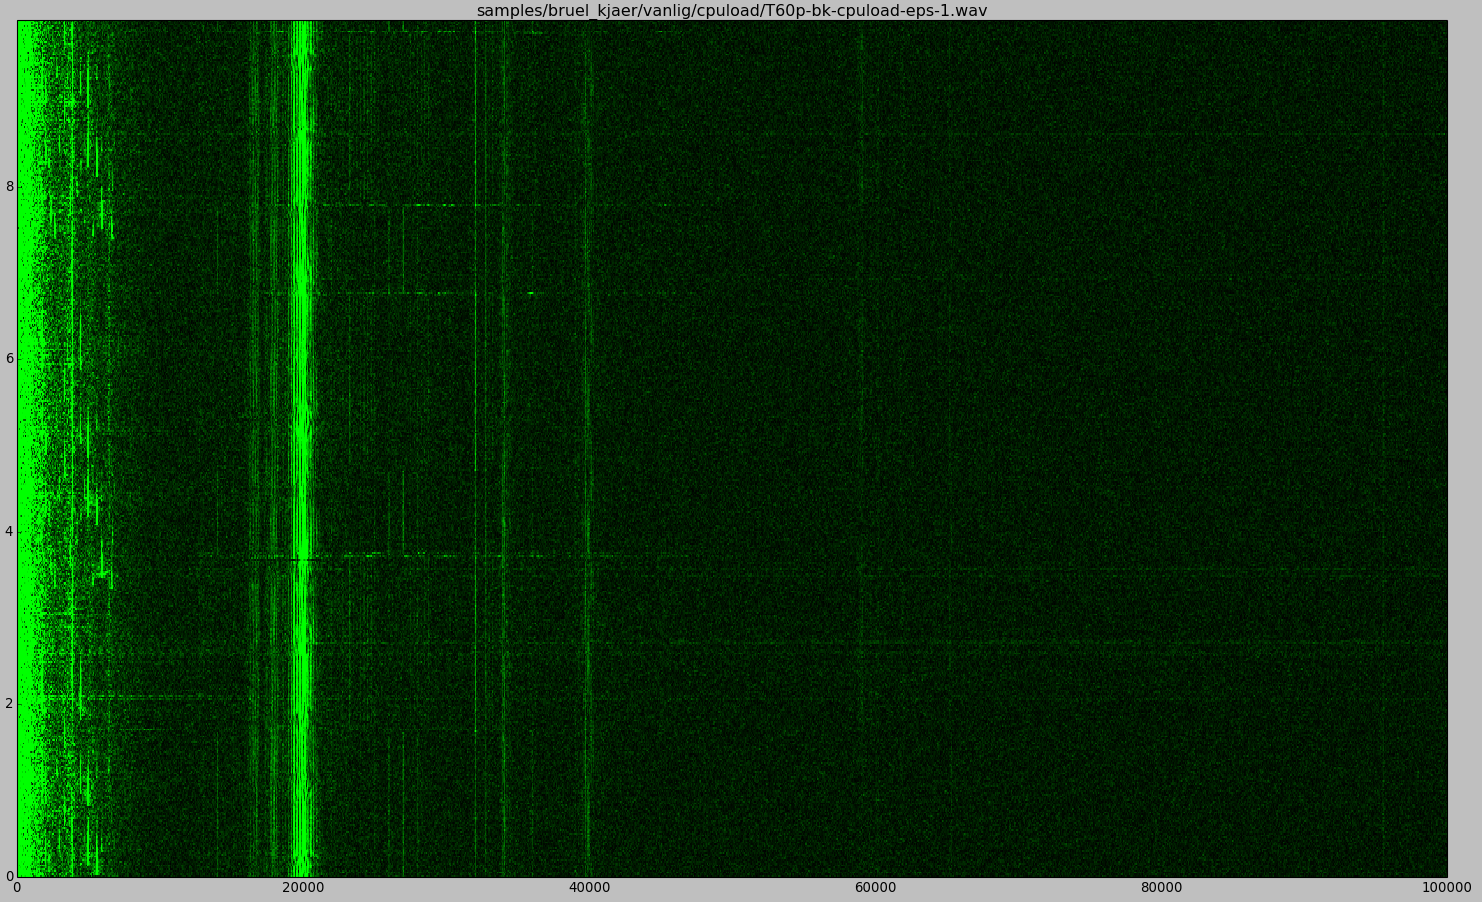
\includegraphics[width=1\linewidth]{T60p-bk-cpuload-eps-1.png}
	    \caption{With power adopter}
	    \label{fig:T60p-bk-cpuload-eps-1-1a}
    \end{subfigure}
    \begin{subfigure}{0.5\textwidth}
	    \centering
	    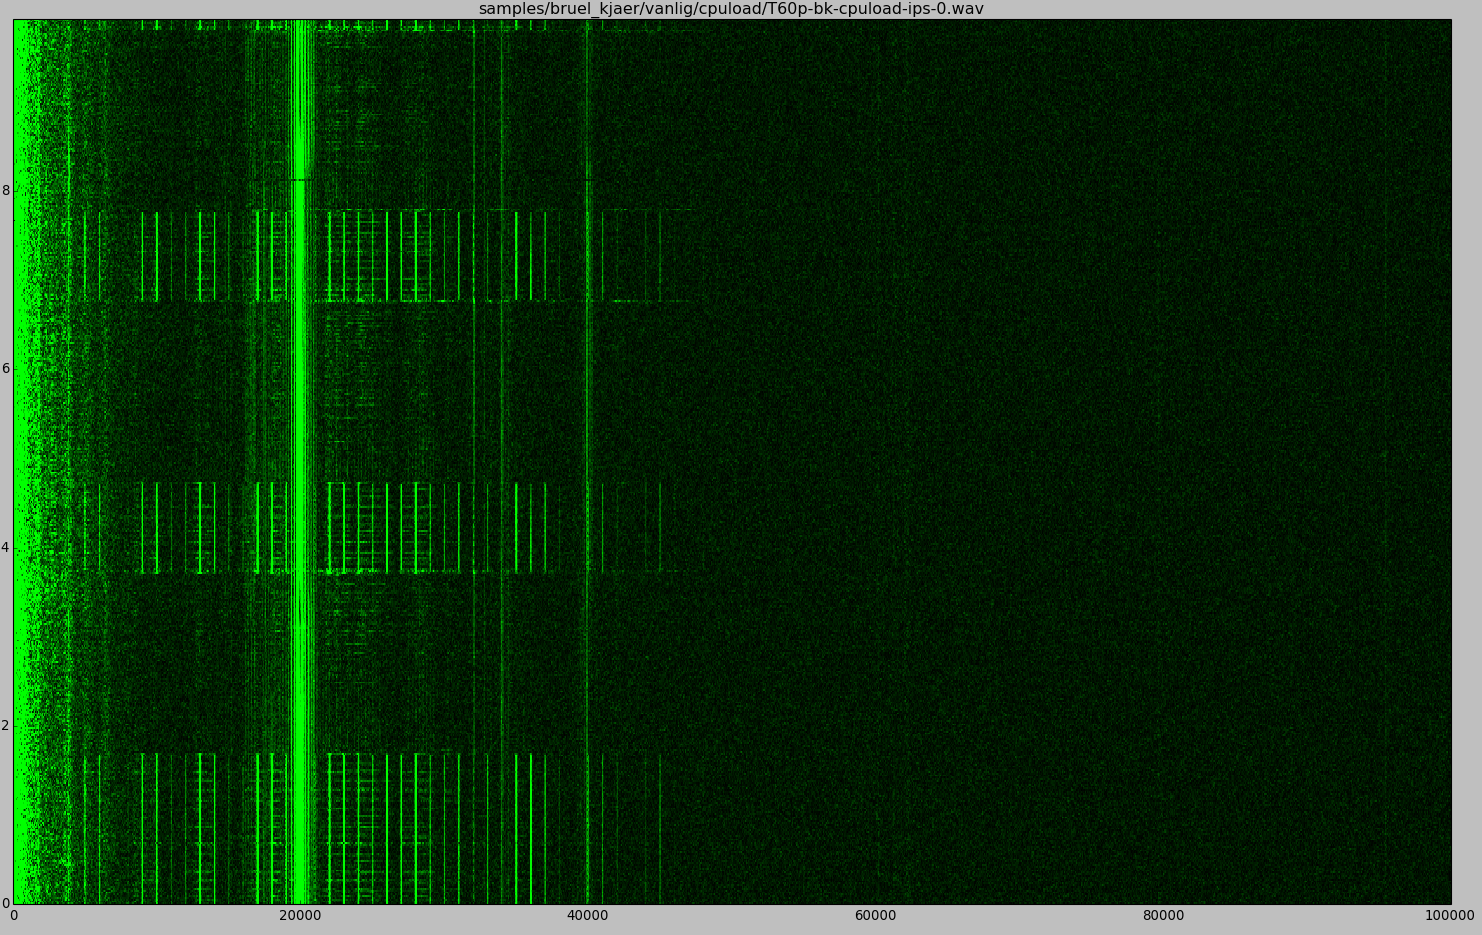
\includegraphics[width=1\linewidth]{T60p-bk-cpuload-ips-0.png}
	    \caption{Running on battery power}
	    \label{fig:T60p-bk-cpuload-ips-0-1b}
    \end{subfigure}
    \caption{Acoustic recording (Vertical axis: 10 sec. Horizontal axis: 0-100kHz) of the Lenovo T60p when running a full CPU load described in~\autoref{chp4:sec:cpu_load}. The recordings was made using the Brüel\&Kjær 4939 configuration specified in~\autoref{ch3:sec:bruel_kjaer_configuration}. }
	\label{fig:T60p-bk-cpuload}
\end{figure}


%==============
% D430 CPULOAD
%==============
\subsection{Results from Dell D430 - CPU load}\label{chp5:subsec:d430_bk_results_cpuload}

%================================
% D430 Anechoic chamber  CPULOAD
%================================
The~\autoref{fig:D430-ekkofritt-bk-cpuload-eps-1} is the results from the running CPU load on the Dell 430 in the anechoic chamber. 
\begin{figure}[ht]
    \centering
    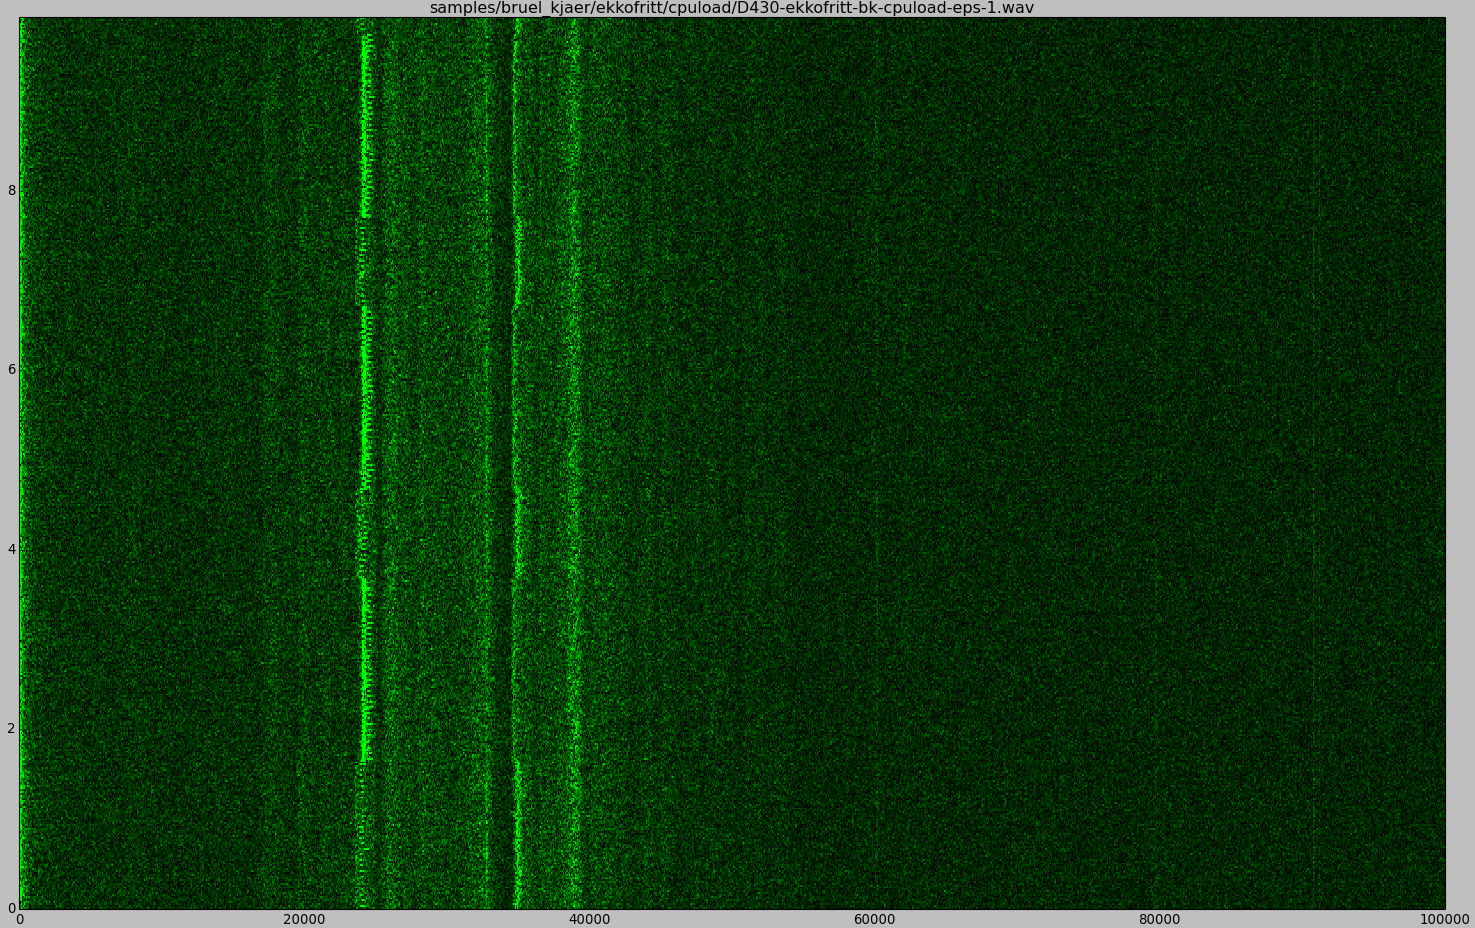
\includegraphics[width=0.7\linewidth]{D430-ekkofritt-bk-cpuload-eps-1.png}
    \caption{Acoustic recording (Vertical axis: 10 sec. Horizontal axis: 0-100kHz) of the Dell D430 when running a full CPU load described in~\autoref{chp4:sec:cpu_load}. The recording was made in an anechoic chamber using the Brüel\&Kjær 4939 configuration specified in~\autoref{ch3:sec:bruel_kjaer_configuration}. }
    \label{fig:D430-ekkofritt-bk-cpuload-eps-1}
\end{figure}


%=================
% T60p Decryption
%=================
\subsection{Results from Lenovo T60p - Decryption}\label{chp5:subsec:t60p_bk_results_decryption}

%===============================
% T60p Anechoic chamber DECRYPT
%===============================
The~\autoref{fig:T60p-ekkofritt-bk-decrypt-ips-3} is the results from the running decryption on the Lenovo T60p in the anechoic chamber. 
\begin{figure}[ht]
    \centering
    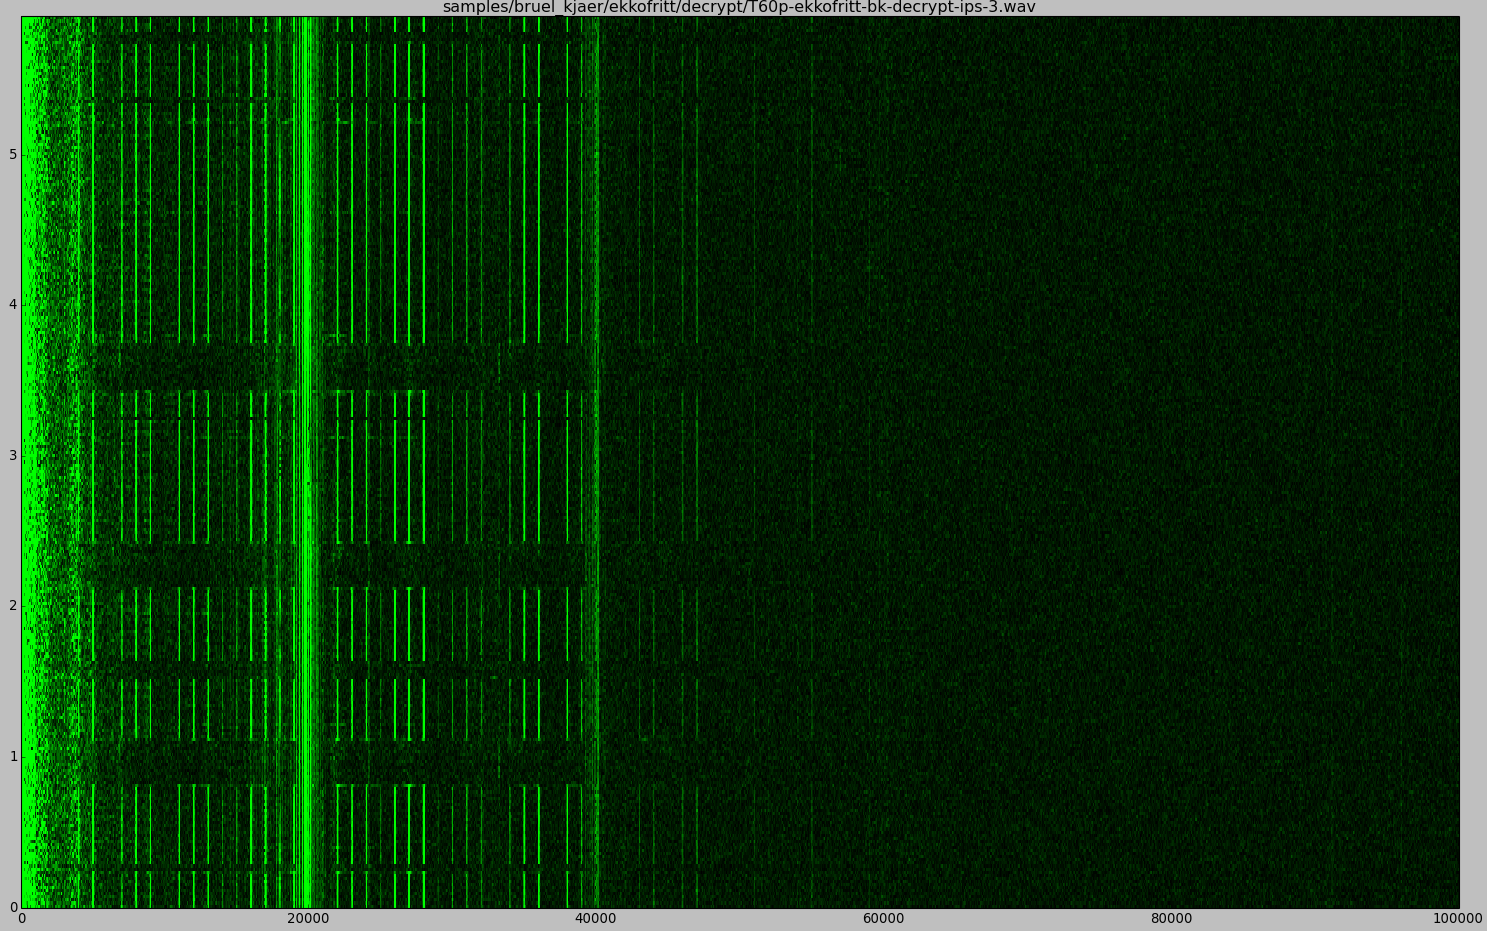
\includegraphics[width=0.7\linewidth]{T60p-ekkofritt-bk-decrypt-ips-3.png}
    \caption{Acoustic recording (Vertical axis: 6 sec. Horizontal axis: 0-100kHz) of the Lenovo T60p when running a decryption described in~\autoref{chp4:sec:decryption}. The recording was made in an anechoic chamber using the Brüel\&Kjær 4939 configuration specified in~\autoref{ch3:sec:bruel_kjaer_configuration}. }
    \label{fig:T60p-ekkofritt-bk-decrypt-ips-3}
\end{figure}

%=================
% D430 Decryption
%=================
\subsection{Results from Dell D430 - Decryption}\label{chp5:subsec:d430_bk_results_cpuload}

%================================
% D430 Anechoic chamber  DECRYPT
%================================
The~\autoref{fig:D430-ekkofritt-bk-decrypt-eps-0} is the results from the running decryption on the Dell 430 in the anechoic chamber. 
\begin{figure}[ht]
    \centering
    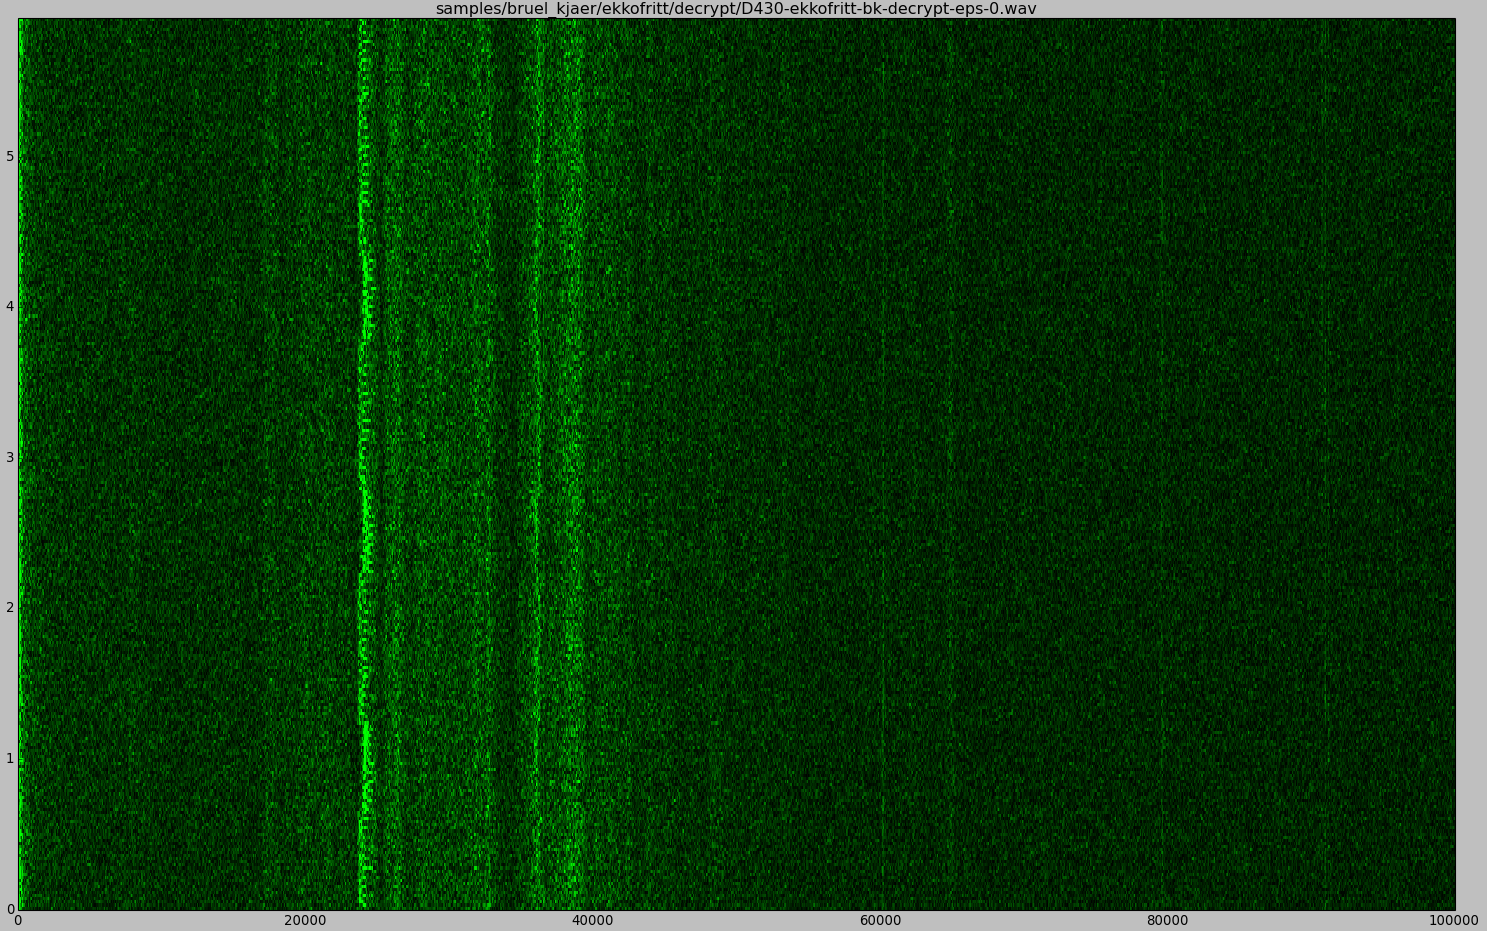
\includegraphics[width=0.7\linewidth]{D430-ekkofritt-bk-decrypt-eps-0.png}
    \caption{Acoustic recording (Vertical axis: 6 sec. Horizontal axis: 0-100kHz) of the Dell D430 when running a decryption described in~\autoref{chp4:sec:decryption}. The recording was made in an anechoic chamber using the Brüel\&Kjær 4939 configuration specified in~\autoref{ch3:sec:bruel_kjaer_configuration}.}
    \label{fig:D430-ekkofritt-bk-decrypt-eps-0}
\end{figure}


%=============================
% D430 Anechoic chamber  IDLE
%=============================
The~\autoref{fig:D430-ekkofritt-bk-idle-eps-1} is the results from the running idle on the Dell 430 in the anechoic chamber. 
\begin{figure}[ht]
    \centering
    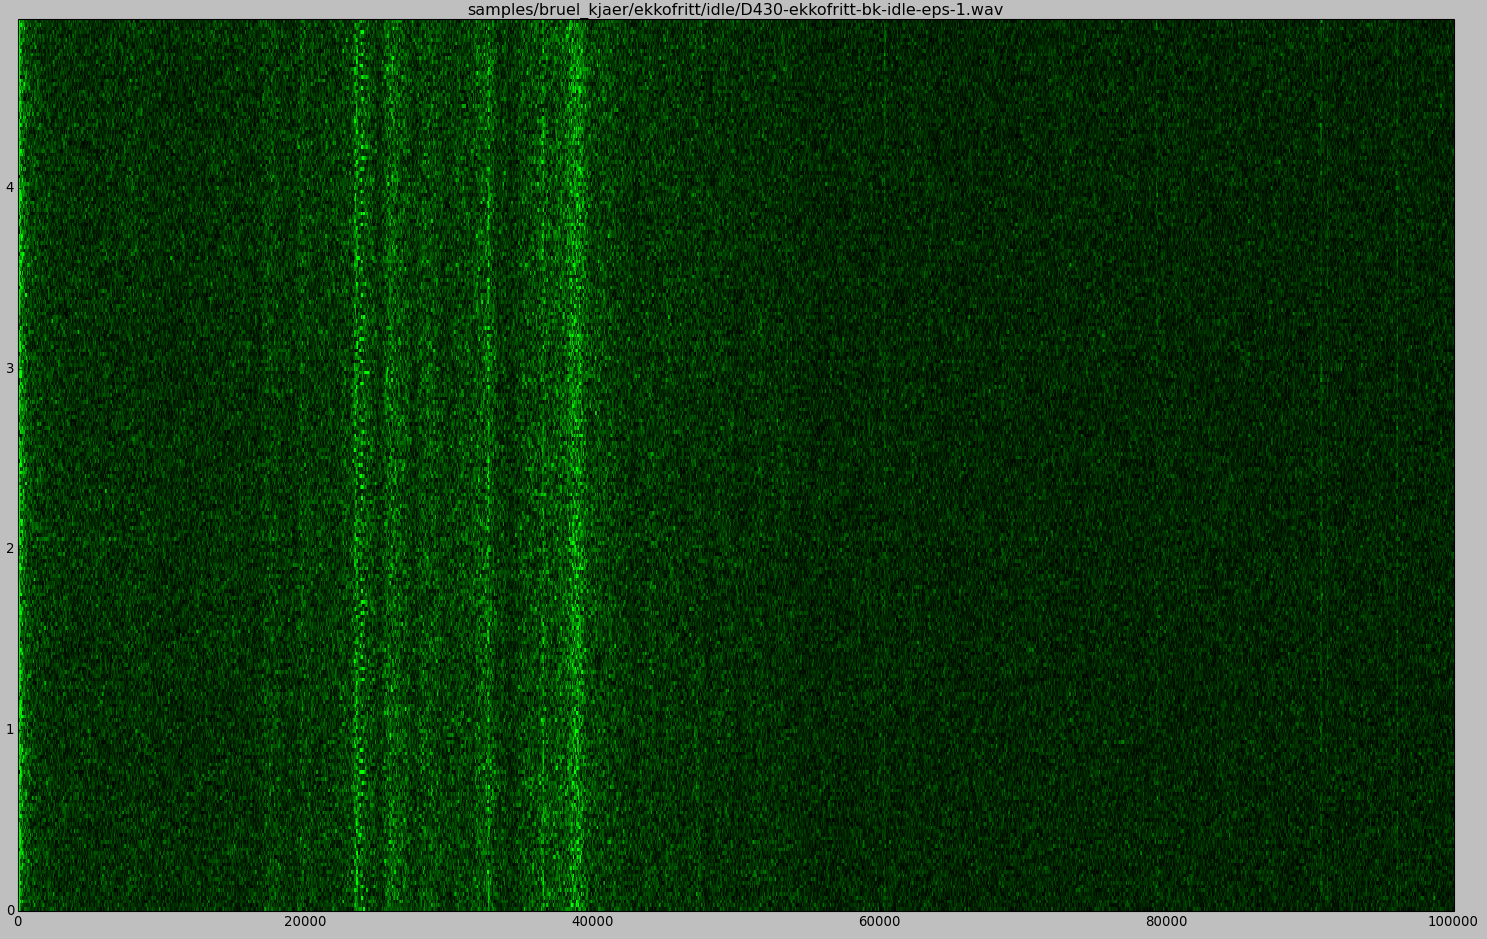
\includegraphics[width=0.7\linewidth]{D430-ekkofritt-bk-idle-eps-1.png}
    \caption{Acoustic recording (Vertical axis: 5 sec. Horizontal axis: 0-100kHz) of the Dell D430 when idle. The recording was made in an anechoic chamber using the Brüel\&Kjær 4939 configuration specified in~\autoref{ch3:sec:bruel_kjaer_configuration}. }
    \label{fig:D430-ekkofritt-bk-idle-eps-1}
\end{figure}

%=====================
% Rasberry PI
%=====================
\subsection{Results from Rasberry PI}\label{chp5:subsec:rb_bk_results}
All results from the Rasberry PI are inconclusive. 
I.e. we are not able to interpret any of the recordings and relate them to the operations we performed.

\section{Microinstructions comparison}

\begin{figure}[ht]
    \centering
    \begin{subfigure}{0.32\textwidth}
        \centering
        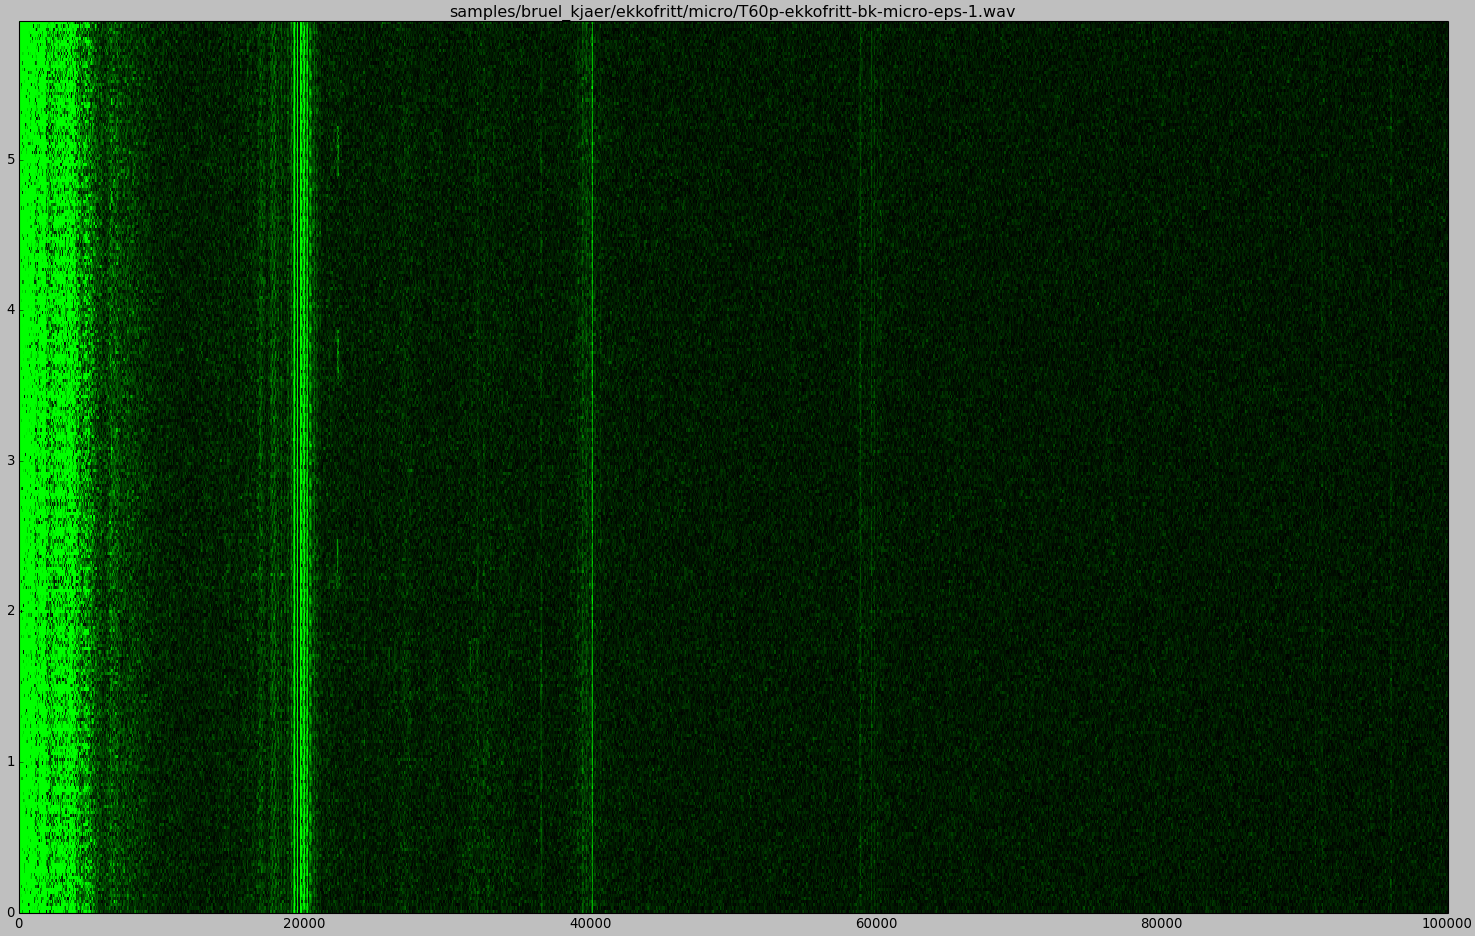
\includegraphics[width=1\linewidth]{T60p-ekkofritt-bk-micro-eps-1.png}
        \caption{Lenovo T60p}
        \label{fig:comparison_T60p-ekkofritt-bk-micro-eps-1}
    \end{subfigure}
    \begin{subfigure}{0.32\textwidth}
        \centering
        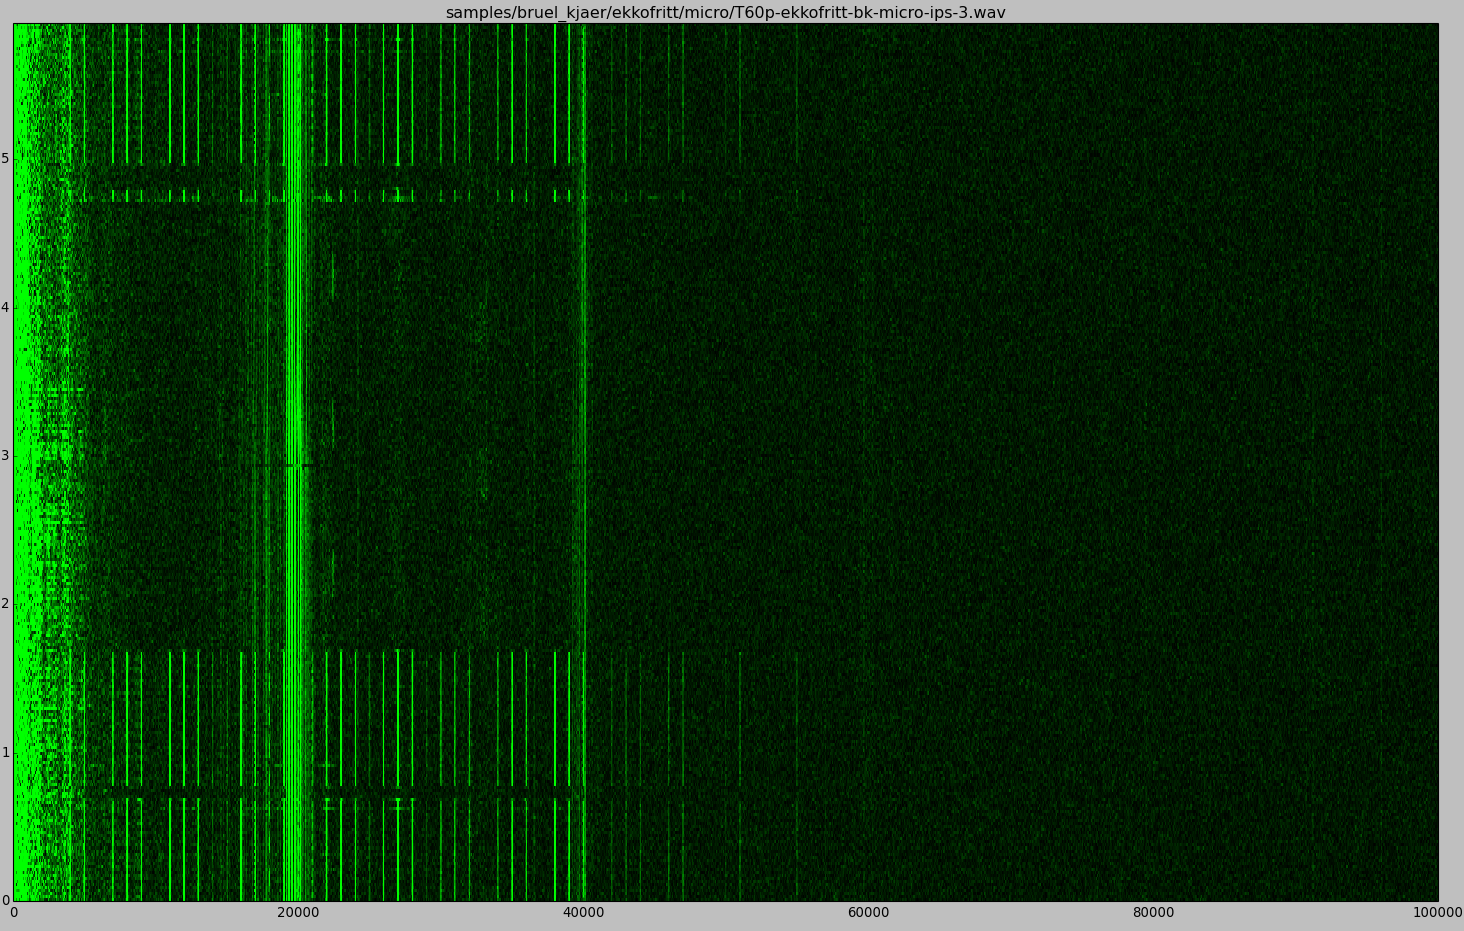
\includegraphics[width=1\linewidth]{T60p-ekkofritt-bk-micro-ips-3.png}
        \caption{Lenovo T60p}
        \label{fig:comparison_T60p-ekkofritt-bk-micro-ips-3}
    \end{subfigure}
    \begin{subfigure}{0.32\textwidth}
        \centering
        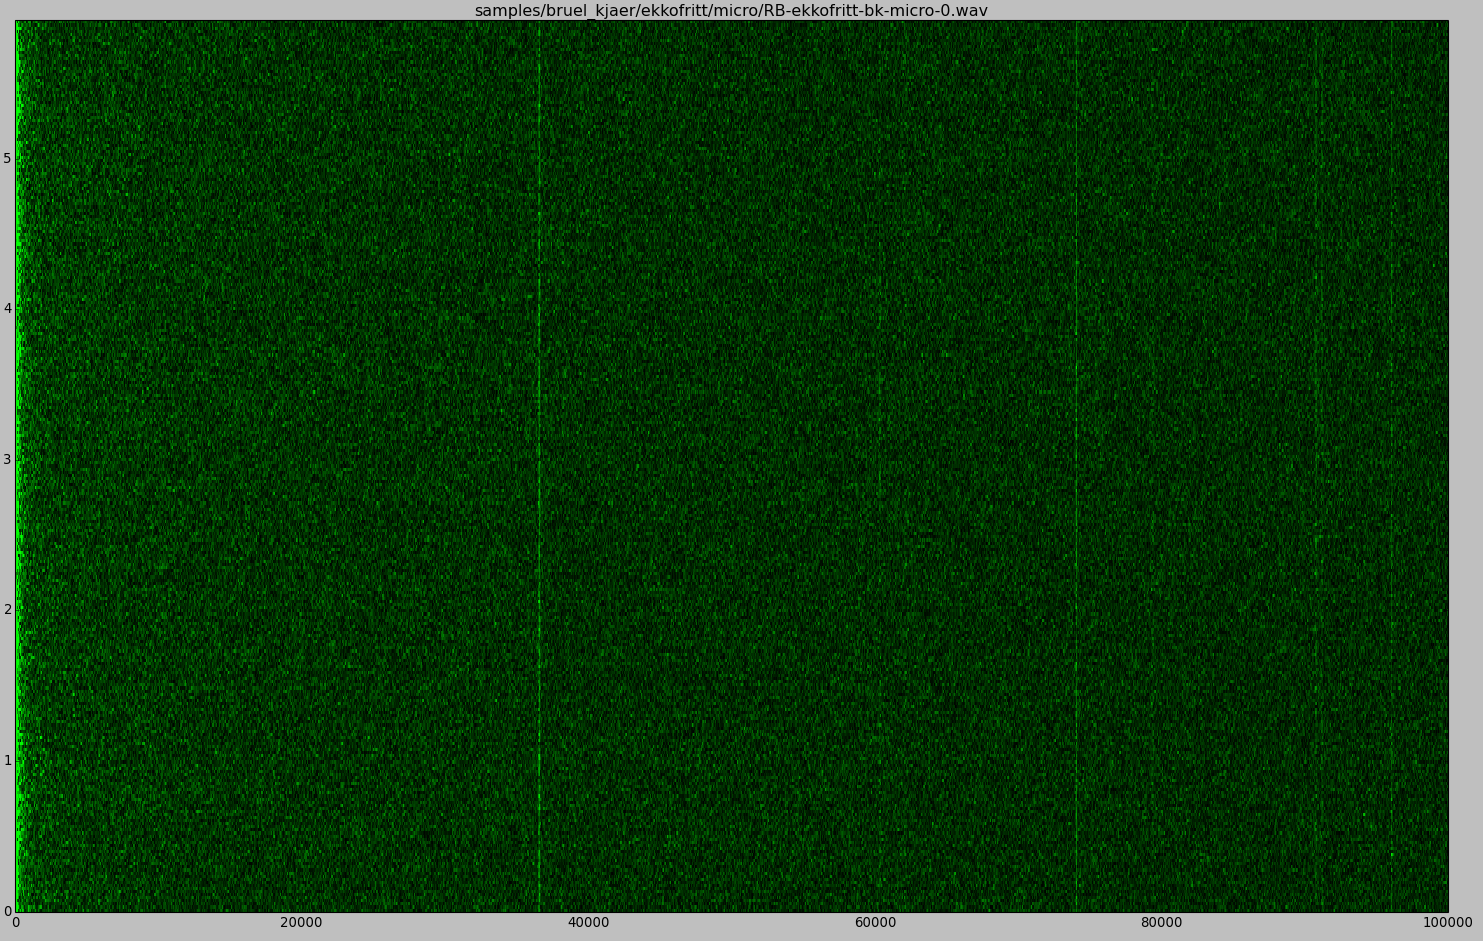
\includegraphics[width=1\linewidth]{RB-ekkofritt-bk-micro-0.png}
        \caption{Rasberry PI}
        \label{fig:comparison_RB-ekkofritt-bk-micro-0}
    \end{subfigure}
    \begin{subfigure}{0.32\textwidth}
        \centering
        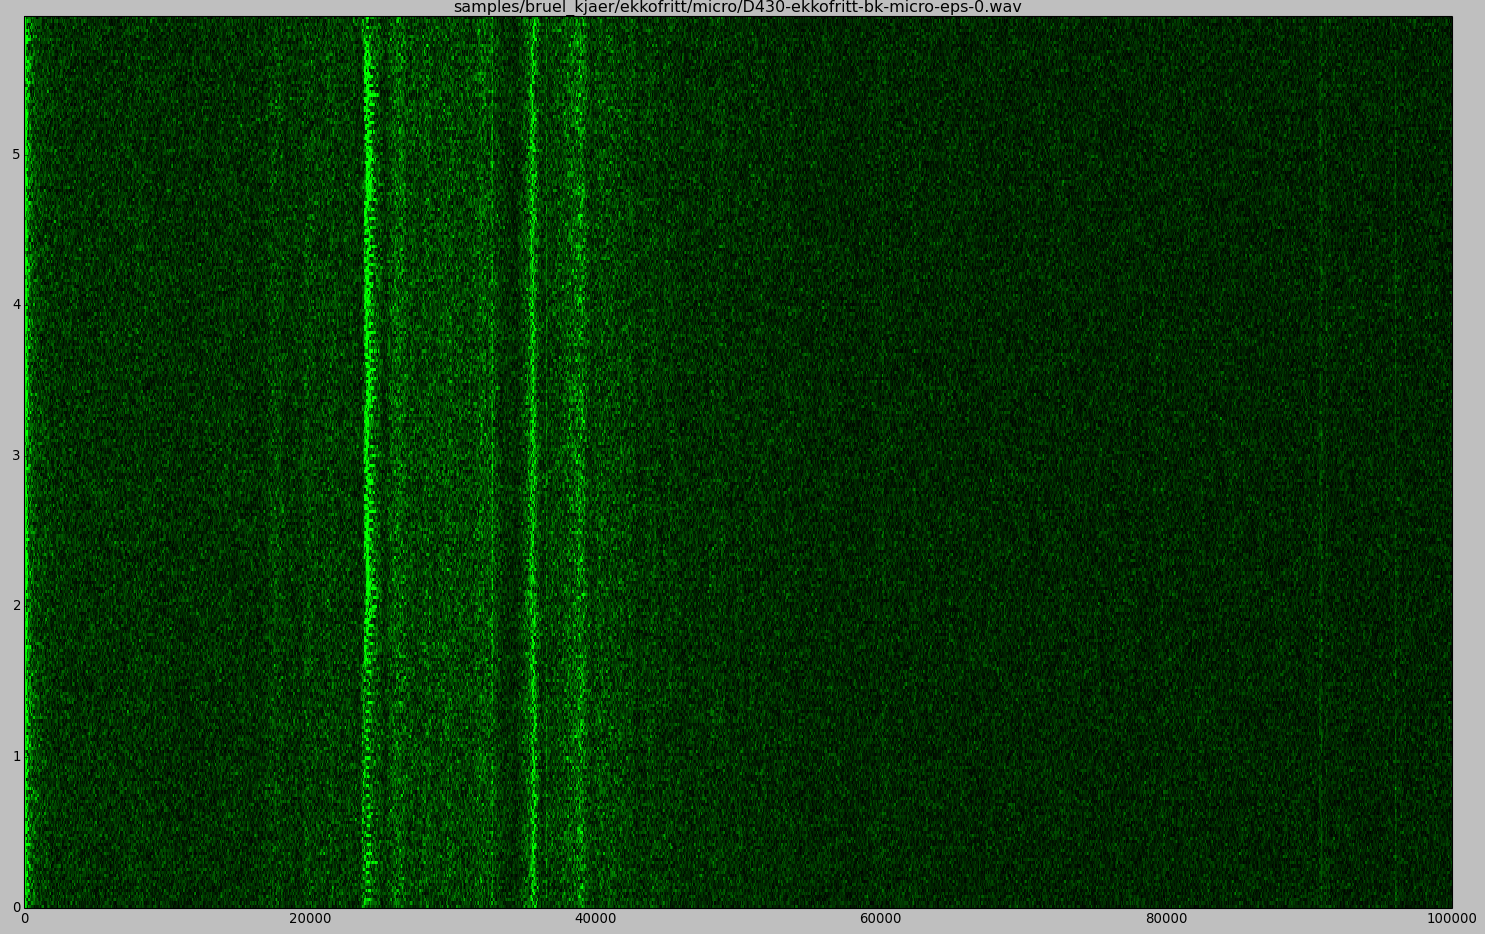
\includegraphics[width=1\linewidth]{D430-ekkofritt-bk-micro-eps-0.png}
        \caption{Dell 430}
        \label{fig:comparison_D430-ekkofritt-bk-micro-eps-0}
    \end{subfigure}
    \begin{subfigure}{0.32\textwidth}
        \centering
        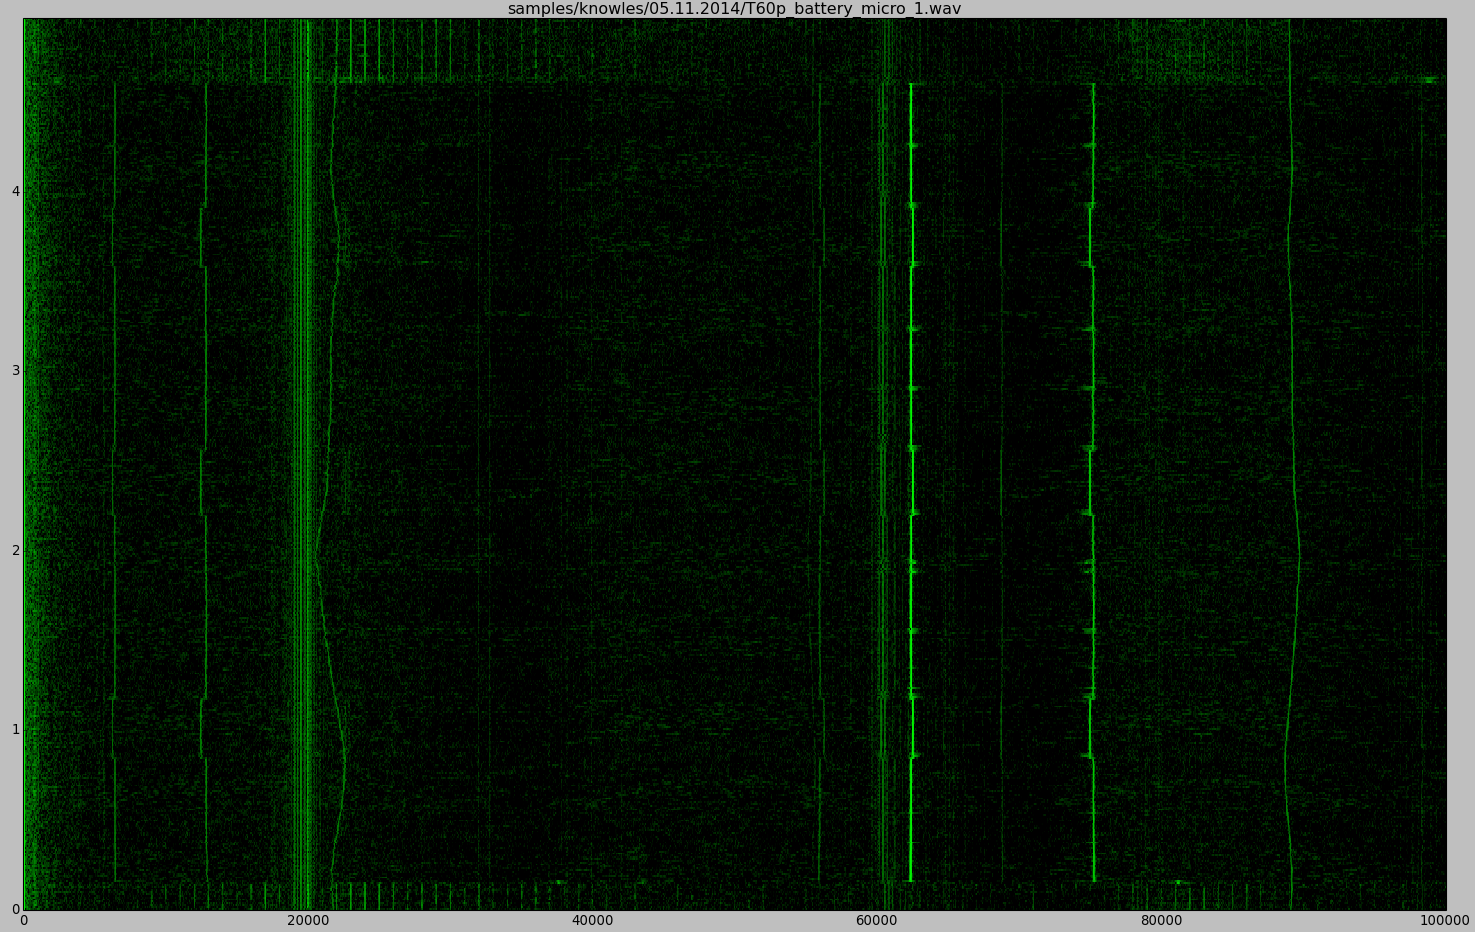
\includegraphics[width=1\linewidth]{T60p-knowles-micro-ips-0.png}
        \caption{Lenovo T60p}
        \label{fig:comparison_T60p-knowles-micro-ips-0}
    \end{subfigure}
    \begin{subfigure}{0.32\textwidth}
        \centering
        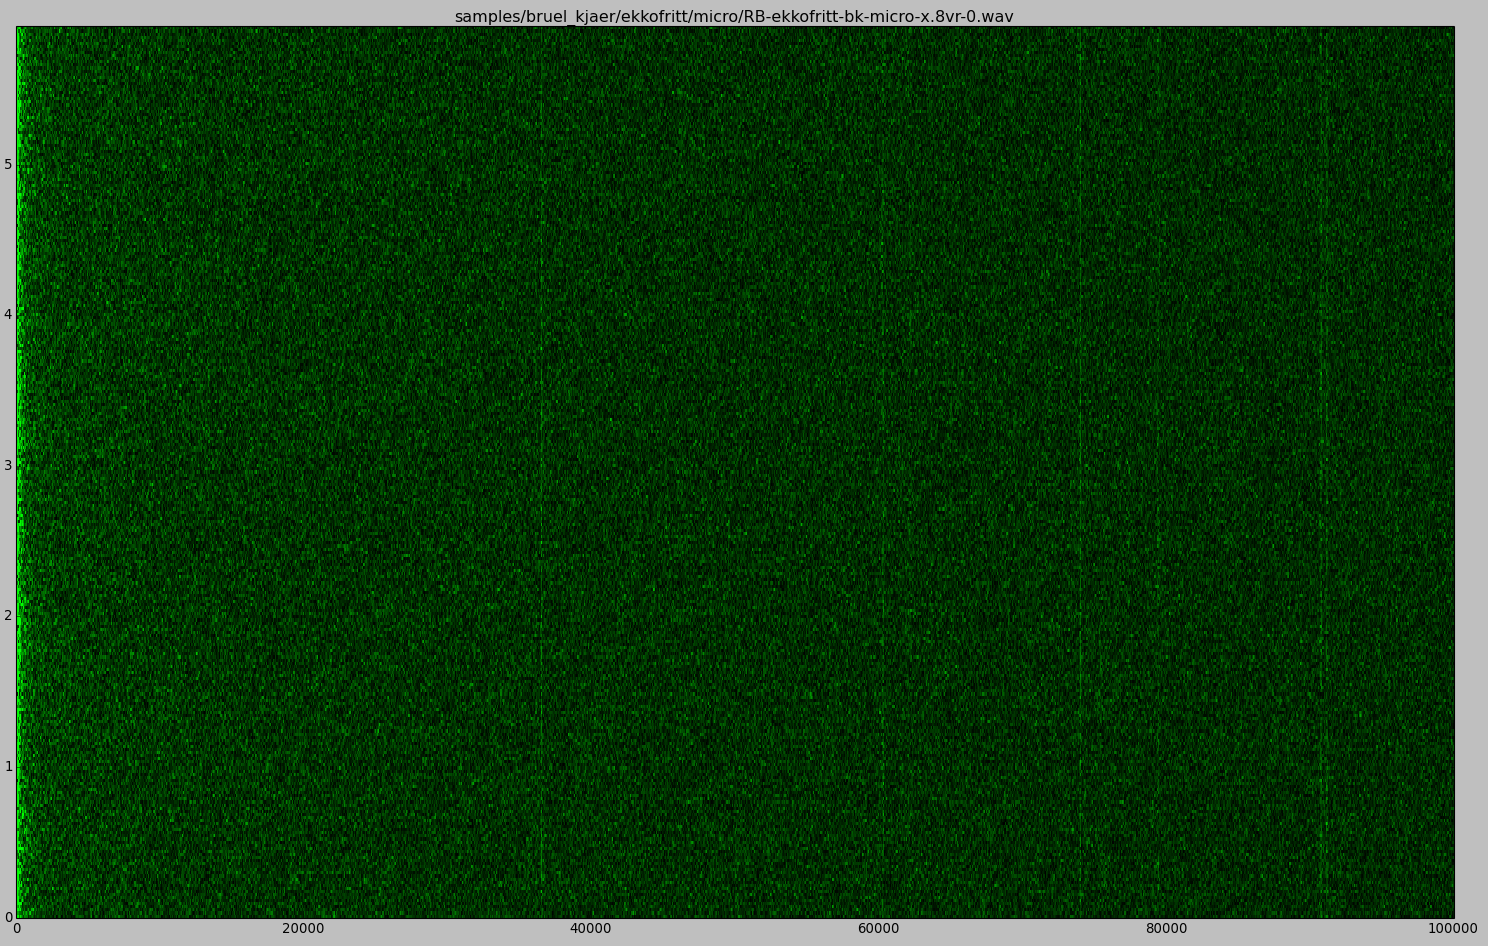
\includegraphics[width=1\linewidth]{RB-ekkofritt-bk-micro-x-8vr-0.png}
        \caption{Rasberry PI}
        \label{fig:comparison_RB-ekkofritt-bk-micro-x-8vr-0}
    \end{subfigure}
    \caption{
    ~\autoref{fig:comparison_T60p-ekkofritt-bk-micro-eps-1} is the T60p with Brüel\&Kjær with power adopter.
    ~\autoref{fig:comparison_T60p-ekkofritt-bk-micro-ips-3} is the T60p with Brüel\&Kjær running on battery power.
    ~\autoref{fig:comparison_RB-ekkofritt-bk-micro-0} is the Rasberry PI with Brüel\&Kjær.
    ~\autoref{fig:comparison_D430-ekkofritt-bk-micro-eps-0} is the Dell D430 with Brüel\&Kjær running on battery power.
    ~\autoref{fig:comparison_T60p-knowles-micro-ips-0} is the T60p with Knowles running on battery power.
    ~\autoref{fig:comparison_RB-ekkofritt-bk-micro-x-8vr-0} is the Rasberry PI on the power input with Brüel\&Kjær.}
    \label{fig:comparison_micorinstructions}
\end{figure}